% Document template suitable for use as a LaTeX master-file 
% for thesis works in University of Turku Department of Computing
%
% Technical usage guide: https://tech.utugit.fi/soft/thesis/doc/doc/overview/
% 

\documentclass[language=english,version=final,mainfont=none,sharelatex=false,pdfaconformance=none]{utuftthesis}
\setcounter{secnumdepth}{2}
\setcounter{tocdepth}{2}
\usepackage{float}
\usepackage[caption=false]{subfig}
\usepackage{amsmath}
\usepackage{booktabs}

% Define the algorithm environment
\providecommand\textquotedblplain{%
  \bgroup\addfontfeatures{Mapping=}\char34\egroup}
\providecommand{\tabularnewline}{\\}
\floatstyle{ruled}
\newfloat{algorithm}{tbp}{loa}
\providecommand{\algorithmname}{Algorithm}
\floatname{algorithm}{\protect\algorithmname}

\addbibresource{Bibliografia.bib}

\begin{document}

\pubyear{2026}
\pubmonth{1}
\publab{Bioinformatics}
\publaben{Bioinformatics}
\pubtype{msc}
\title{Microbiome-Based Body Mass Index Prediction: A Machine Learning Pipeline for Large-Scale Metagenomic Data}
\author{Sadia Zaman}

\maketitle
% ============================================================
% ABSTRACT
% University of Turku, Faculty of Technology
% MSc Thesis - Microbiome-Based BMI Prediction
% ============================================================

\begin{abstract}

The human gut microbiome has emerged as a key modulator of host metabolism and body composition. This thesis investigates whether gut microbial composition, assessed through shotgun metagenomics, can predict Body Mass Index (BMI) using supervised machine learning. A reproducible Nextflow pipeline was developed and applied to 17,903 human samples from the Metalog consortium—one of the largest metagenomic cohorts assembled for this purpose.

Four machine learning algorithms were benchmarked: Elastic Net (linear baseline), Random Forest, XGBoost, and Support Vector Machine. Random Forest achieved the highest predictive performance ($R^2 = 0.325$), more than doubling the linear baseline ($R^2 = 0.14$), demonstrating that the microbiome-BMI relationship is fundamentally non-linear. Feature importance analysis identified \emph{Adlercreutzia equolifaciens}, \emph{Roseburia lenta}, and several uncharacterized species as leading predictors, offering candidates for mechanistic investigation.

A 1\% prevalence filter reduced dimensionality by 83\% (10,701 to 1,799 features) with negligible accuracy loss, dramatically improving computational efficiency. Saturation analysis revealed diminishing returns beyond 10,000 samples, providing practical guidance for resource-constrained studies. The pipeline, trained exclusively on microbial features without demographic covariates, establishes a microbiome-only baseline for BMI prediction.

These findings confirm that the gut ecosystem encodes meaningful metabolic information accessible through standard machine learning pipelines on consumer-grade hardware. The reproducible workflow and identified taxa provide a foundation for translating microbial insights into precision nutrition and personalized medicine.

\end{abstract}




% mandatory
\tableofcontents

% if you want a list of figures
\listoffigures

% if you want a list of tables
\listoftables

% The thesis starts here.

% ============================================================
% CHAPTER 1: INTRODUCTION
% University of Turku, Faculty of Technology
% MSc Thesis - Microbiome-Based BMI Prediction
% Author: Sadia Zaman
% ============================================================

\chapter{Introduction}
\label{ch:introduction}

The human gut microbiome---the vast consortium of bacteria, archaea, viruses, and fungi colonizing the gastrointestinal tract---has emerged as a critical determinant of host metabolism and body composition. With the global prevalence of obesity exceeding 650 million adults and its classification as a pandemic by the World Health Organization, the scientific community has turned its attention toward the gut ecosystem as both a diagnostic reservoir and a therapeutic target \cite{who2021obesity}.

\section{Motivation and Problem Statement}

Traditional epidemiological models of obesity rely on demographic and behavioral covariates: age, sex, caloric intake, and physical activity. While these factors explain a substantial portion of variance in Body Mass Index (BMI), they fail to account for the striking inter-individual variability observed even among subjects with identical lifestyles. This ``metabolic individuality'' has catalyzed interest in the microbiome as a missing explanatory layer.

Recent large-scale metagenomic studies have demonstrated that gut microbial composition correlates with host phenotypes including insulin resistance, inflammation, and adiposity \cite{turnbaugh2006obesity}. However, most published work remains correlative, and the transition from association to prediction---from understanding \emph{which} bacteria correlate with BMI to building models that \emph{forecast} BMI from taxonomic profiles---remains an active frontier.

\section{Research Questions}

This thesis addresses three interconnected research questions:

\begin{enumerate}
    \item \textbf{Predictive Capacity:} Can machine learning models trained exclusively on gut microbiome composition predict host BMI with clinically meaningful accuracy?
    \item \textbf{Algorithm Selection:} How do linear models (Elastic Net) compare to non-linear ensemble methods (Random Forest, XGBoost, SVM) in capturing the complex, high-dimensional structure of microbiome data?
    \item \textbf{Scalability and Efficiency:} What preprocessing strategies (e.g., prevalence filtering) and sample sizes are sufficient to achieve robust performance on consumer-grade hardware?
\end{enumerate}

\section{Contributions}

This work makes the following contributions:

\begin{itemize}
    \item A reproducible, end-to-end Nextflow pipeline for microbiome-based phenotype prediction, designed for portability between local workstations and high-performance computing clusters.
    \item A rigorous benchmark of four machine learning algorithms on 17,903 human gut metagenomes from the Metalog consortium, representing one of the largest such analyses to date.
    \item A saturation analysis quantifying the relationship between sample size and predictive performance, providing practical guidance for future studies with resource constraints.
    \item Identification of specific bacterial taxa (e.g., \emph{Adlercreutzia equolifaciens}, \emph{Roseburia lenta}) as top predictors of BMI, offering candidates for downstream mechanistic investigation.
\end{itemize}

\section{Thesis Structure}

The remainder of this thesis is organized as follows. Chapter~\ref{ch:literature} surveys the scientific literature on microbiome-obesity associations and machine learning applications in metagenomics. Chapter~\ref{ch:methods} details the dataset, preprocessing pipeline, and modeling framework. Chapter~\ref{ch:results} presents the experimental results, including model comparisons and feature importance analysis. Chapter~\ref{ch:discussion} interprets the findings in the context of prior work and discusses limitations. Finally, Chapter~\ref{ch:conclusion} summarizes the contributions and outlines directions for future research.

% ============================================================
% CHAPTER 2: LITERATURE REVIEW
% University of Turku, Faculty of Technology
% MSc Thesis - Microbiome-Based BMI Prediction
% ============================================================

\chapter{Literature Review}
\label{ch:literature}

This chapter surveys the scientific foundations of microbiome-based phenotype prediction, organized into three thematic sections: the biological basis of gut-obesity interactions, computational approaches to microbiome analysis, and the current state of machine learning in metagenomics.

\section{The Gut Microbiome and Host Metabolism}

The human gastrointestinal tract harbors approximately $10^{13}$ microbial cells---a population rivaling the count of human somatic cells---encoding a collective genome (the ``microbiome'') orders of magnitude larger than the host genome \cite{sender2016revised}. This microbial consortium performs metabolic functions inaccessible to human enzymes, including the fermentation of dietary fiber into short-chain fatty acids (SCFAs), the synthesis of vitamins B and K, and the biotransformation of bile acids \cite{rowland2018gut}.

\subsection{Early Observations: The Firmicutes/Bacteroidetes Hypothesis}

The seminal work of Turnbaugh et al.\ (2006) demonstrated that germ-free mice colonized with microbiota from obese donors gained significantly more fat mass than those receiving microbiota from lean donors, despite identical caloric intake \cite{turnbaugh2006obesity}. This landmark study proposed the Firmicutes/Bacteroidetes (F/B) ratio as a biomarker for obesity, with obese individuals exhibiting elevated Firmicutes relative to Bacteroidetes.

However, subsequent meta-analyses have challenged the universality of this ratio. A systematic review encompassing 23 independent cohorts found no consistent association between the F/B ratio and BMI after controlling for age, sex, and geographic origin \cite{magne2020firmicutes}. The discrepancy likely reflects methodological heterogeneity---differences in DNA extraction protocols, sequencing platforms, and taxonomic classification pipelines---as well as the profound influence of diet, which can shift gut composition within 24 hours \cite{david2014diet}.

\subsection{Beyond Phylum-Level Markers: Species-Specific Associations}

Contemporary research has moved beyond coarse taxonomic summaries toward species- and strain-level resolution. A 2024 meta-analysis pooling metagenomic data from over 3,300 samples across 17 countries identified 25 bacterial species reproducibly associated with obesity, including:\cite{NIHMBMI2024}

\begin{itemize}
    \item \textbf{\emph{Akkermansia muciniphila}}: Consistently depleted in obese subjects; implicated in mucin degradation and gut barrier integrity.
    \item \textbf{\emph{Bifidobacterium longum}}: Negatively correlated with BMI; produces acetate and lactate with anti-inflammatory properties.
    \item \textbf{\emph{Faecalibacterium prausnitzii}}: A major butyrate producer; reduced abundance linked to metabolic inflammation.
\end{itemize}

Importantly, these associations persist after adjusting for confounders, suggesting genuine biological relevance rather than spurious correlation with demographic proxies.

\section{Computational Metagenomics}

\subsection{From Reads to Taxa: The Bioinformatics Pipeline}

Modern metagenomic analysis proceeds through a standardized computational workflow:

\begin{enumerate}
    \item \textbf{Sequencing:} Shotgun metagenomic sequencing generates millions of short DNA reads per sample.
    \item \textbf{Quality Control:} Reads are trimmed to remove adapters and low-quality bases.
    \item \textbf{Taxonomic Profiling:} Tools such as MetaPhlAn4 assign reads to reference genomes, producing relative abundance tables at species resolution \cite{blanco2023metaphlan4}.
    \item \textbf{Downstream Analysis:} Abundance tables serve as input to statistical and machine learning models.
\end{enumerate}

\subsection{Challenges in Microbiome Data}

Microbiome datasets present unique statistical challenges that distinguish them from conventional tabular data:

\begin{itemize}
    \item \textbf{Compositionality:} Relative abundances are constrained to sum to unity, inducing spurious negative correlations between taxa.
    \item \textbf{Sparsity:} The majority of taxa are absent (zero abundance) in the majority of samples, with zero-inflation rates often exceeding 90\%.
    \item \textbf{High Dimensionality:} A typical dataset may contain thousands of species but only hundreds of samples, creating a $p >> n$ scenario prone to overfitting.
\end{itemize}

These characteristics motivate specialized preprocessing---variance filtering, normalization, and transformation---prior to model training.

\section{Machine Learning in Microbiome Research}

\subsection{Algorithm Landscape}

Machine learning applications in metagenomics span classification (e.g., disease vs.\ healthy) and regression (e.g., predicting continuous BMI). The most commonly benchmarked algorithms include:

\textbf{Elastic Net (GLMNet):} A regularized linear model combining L1 (Lasso) and L2 (Ridge) penalties. Elastic Net excels at feature selection in high-dimensional settings but assumes additive, linear effects---a potentially restrictive assumption for microbiome interactions \cite{zou2005regularization}.

\textbf{Random Forest:} An ensemble of decision trees trained on bootstrap samples with random feature subsets. Random Forest captures non-linear relationships and interactions without explicit specification, and provides intrinsic feature importance via permutation or Gini impurity \cite{breiman2001random}.

\textbf{XGBoost (Gradient Boosting):} A sequential ensemble method that iteratively corrects errors from previous trees. XGBoost often achieves state-of-the-art performance on tabular data and offers fine-grained hyperparameter control, though at increased computational cost \cite{chen2016xgboost}.

\textbf{Support Vector Machine (SVM):} A kernel-based classifier that finds optimal separating hyperplanes. While powerful for binary classification, SVM scales poorly ($O(n^3)$) with sample size, limiting its applicability to large metagenomic cohorts.

\subsection{Benchmark Studies}

Comparative evaluations of these algorithms on microbiome data have yielded nuanced conclusions. A systematic benchmark across 29 human microbiome datasets found that XGBoost, Random Forest, and Elastic Net exhibited statistically comparable performance for classification tasks, with algorithm choice less impactful than feature engineering and data quality \cite{topccuouglu2020framework}. Similarly, studies on Inflammatory Bowel Disease diagnosis demonstrated that non-linear models (Random Forest, XGBoost) significantly outperformed linear baselines, achieving Matthews Correlation Coefficients exceeding 0.7 \cite{ibdbenchmark2024}.

For regression tasks---such as predicting age or BMI---tree-based ensembles dominate the literature. Random Forest adapts naturally to regression by averaging predictions across trees, while XGBoost minimizes squared-error loss through gradient descent. A comparative analysis under varying noise levels found Random Forest more robust to discontinuous response functions, while XGBoost excelled with smooth, continuous patterns \cite{regressionbenchmark2023}.

\subsection{The mikropml Framework}

This thesis employs the \texttt{mikropml} R package, developed by the Schloss Laboratory, which provides a standardized interface for microbiome machine learning \cite{mikropml2021}. The package implements:

\begin{itemize}
    \item Automated preprocessing (near-zero variance removal, centering, scaling).
    \item Hyperparameter tuning via cross-validation.
    \item Rigorous train/test separation to prevent data leakage.
\end{itemize}

By abstracting common pitfalls, \texttt{mikropml} enhances reproducibility and comparability across studies.

\section{Summary}

The literature establishes three key premises for this thesis:

\begin{enumerate}
    \item The gut microbiome contains genuine biological signal predictive of host metabolic phenotypes, including BMI.
    \item Traditional biomarkers (e.g., F/B ratio) are unreliable; species-level resolution and large sample sizes are required.
    \item Non-linear ensemble methods (Random Forest, XGBoost) consistently outperform linear baselines on microbiome data, though marginal differences between ensembles diminish with proper tuning.
\end{enumerate}

These insights inform the methodological choices described in Chapter~\ref{ch:methods}.

% ============================================================
% CHAPTER 3: METHODS
% University of Turku, Faculty of Technology
% MSc Thesis - Microbiome-Based BMI Prediction
% ============================================================

\chapter{Methods}
\label{ch:methods}

This chapter describes the dataset, computational pipeline, and experimental design employed in this thesis. All code is publicly available in the accompanying GitHub repository.

\section{Dataset: The Metalog Consortium}

\subsection{Data Sources and Merging}

The analysis draws on two complementary data products from the Metalog project, a large-scale aggregation of human gut metagenomes:

\begin{itemize}
    \item \textbf{Metadata Table} (\texttt{human\_extended\_wide.tsv}): Contains sample identifiers and phenotypic variables including age, sex, weight, height, and calculated BMI.
    \item \textbf{Taxonomic Profiles} (\texttt{human\_metaphlan4\_species.tsv}): Species-level relative abundances generated by MetaPhlAn4 from shotgun metagenomic reads.
\end{itemize}

Tables were merged on the common \texttt{sample\_id} key using an inner join, retaining only samples present in both sources. The merged dataset comprises \textbf{17,903 human samples} spanning diverse geographic origins, dietary patterns, and health statuses.

\subsection{Target Variable}

The prediction target is Body Mass Index (BMI), defined as:
\begin{equation}
\text{BMI} = \frac{\text{Weight (kg)}}{\text{Height (m)}^2}
\end{equation}
BMI is treated as a continuous outcome for regression modeling. The distribution in the dataset ranges from 14.5 to 58.2 kg/m\textsuperscript{2} with a mean of 25.3 and standard deviation of 5.1.

\subsection{Data Leakage Prevention}

A critical design decision concerns the exclusion of certain predictor variables to prevent data leakage:

\begin{itemize}
    \item \textbf{Weight:} Excluded because BMI is derived directly from weight. Including weight would provide the model with the ``answer'' and yield artificially inflated performance.
    \item \textbf{Age and Sex:} Excluded to isolate the microbial signal. While age and sex are known correlates of both BMI and microbiome composition, including them would conflate demographic prediction with microbiome-based inference. This study aims to establish a \emph{microbiome-only baseline}---demonstrating that gut composition alone contains predictive information about host phenotype.
\end{itemize}

\section{Computational Pipeline}

\subsection{Workflow Management: Nextflow}

The analysis pipeline is implemented in Nextflow, a domain-specific language for data-driven workflows \cite{ditommaso2017nextflow}. Nextflow offers:

\begin{itemize}
    \item \textbf{Reproducibility:} Containerized execution ensures identical results across environments.
    \item \textbf{Portability:} The same code runs on local machines, cloud platforms, and HPC clusters without modification.
    \item \textbf{Parallelism:} Independent tasks (e.g., training different models) execute concurrently, reducing wall-clock time.
\end{itemize}

The pipeline comprises two main processes:

\begin{enumerate}
    \item \texttt{Preprocess}: Loads the merged dataset, applies filters, and prepares data for modeling.
    \item \texttt{TrainModel}: Trains a specified machine learning algorithm and outputs performance metrics.
\end{enumerate}

\subsection{Preprocessing}

Preprocessing is performed using the \texttt{mikropml} R package and proceeds as follows:

\subsubsection{1\% Prevalence Filter}

Bacterial species present in fewer than 1\% of samples (approximately 179 individuals) are removed. This filter eliminates rare taxa unlikely to generalize across populations and substantially reduces dimensionality:

\begin{center}
\textbf{Features: 10,701 $\rightarrow$ 1,799} (83\% reduction)
\end{center}

This aggressive filtering accelerates computation without sacrificing predictive signal, as rare taxa contribute primarily noise to ensemble models.

\subsubsection{Variance Filtering (Top 1000)}

To address the high dimensionality and computational resource constraints, a variance-based feature selection step was implemented. We computed the variance for all 1,799 prevalence-filtered features and retained only the \textbf{Top 1,000 features} with the highest variance. This step reduces noise by eliminating features that show little variation across the population, focusing the model on the most potentially discriminative taxa.

\subsubsection{Centering and Scaling}

The selected 1,000 features are centered (mean = 0) and scaled (standard deviation = 1). Scaling parameters are computed on the training set and applied to the test set to prevent leakage.

\section{Machine Learning Models}

Four algorithms were benchmarked, representing a spectrum from linear to highly non-linear approaches:

\subsection{Elastic Net (GLMNet)}

Elastic Net combines L1 (Lasso) and L2 (Ridge) regularization. It performs implicit feature selection and serves as a linear baseline \cite{zou2005regularization}.

\subsection{Random Forest}

Random Forest constructs an ensemble of $B$ decision trees. We trained the model using 5-fold cross-validation. This bagging strategy decorrelates trees, reducing variance and capturing non-linear interactions \cite{breiman2001random}.

\subsection{XGBoost}

Extreme Gradient Boosting builds trees sequentially, with each tree correcting residuals from the previous iteration. We utilized the \texttt{xgbTree} method in \texttt{caret}, which is highly efficient and robust \cite{chen2016xgboost}.

\subsection{Support Vector Machine (Linear)}

While SVM with a radial basis function (RBF) kernel is powerful, it scales poorly ($O(n^3)$) with sample size. To enable training on the full dataset (18,000 samples) within local hardware memory limits, we employed \textbf{Linear SVM} (\texttt{svmLinear}). This approach finds the optimal separating hyperplane in the feature space with significantly lower computational overhead ($O(n)$) compared to kernel methods.

\section{Evaluation Framework}

\subsection{Cross-Validation}

Model performance is estimated using $k$-fold cross-validation (default $k=5$). The dataset is partitioned into $k$ folds; for each fold, the model trains on $k-1$ folds and evaluates on the held-out fold. Reported metrics represent the mean across folds.

\subsection{Metrics}

For regression tasks, primary metrics include:

\begin{itemize}
    \item \textbf{R-squared ($R^2$):} The proportion of variance explained by the model:
    \begin{equation}
    R^2 = 1 - \frac{\sum_i (y_i - \hat{y}_i)^2}{\sum_i (y_i - \bar{y})^2}
    \end{equation}
    \item \textbf{Root Mean Squared Error (RMSE):} The standard deviation of residuals:
    \begin{equation}
    \text{RMSE} = \sqrt{\frac{1}{n} \sum_i (y_i - \hat{y}_i)^2}
    \end{equation}
\end{itemize}

\subsection{Feature Importance}

For Random Forest, feature importance is quantified via \emph{increase in node purity} (Gini importance). Features splitting nodes effectively---those yielding large reductions in squared error---receive higher importance scores. The top 20 features are reported to identify candidate bacterial taxa for downstream biological investigation.

\section{Saturation Analysis}

To assess the relationship between sample size and performance, a saturation (learning curve) analysis was conducted:

\begin{enumerate}
    \item Subsamples of size $n \in \{1000, 5000, 10000, 15000, 17903\}$ were drawn.
    \item For each subsample, Random Forest was trained with 2-fold cross-validation.
    \item $R^2$ and training time were recorded.
\end{enumerate}

This analysis addresses whether additional samples yield diminishing returns and informs decisions about computational resource allocation.

\section{Hardware and Software}

Experiments were conducted on a consumer-grade Apple MacBook with 8GB RAM. Computationally intensive models (Random Forest on full data) required up to 16 hours of wall-clock time. The Nextflow pipeline is designed for seamless transition to HPC environments for future scaling.

\textbf{Software Stack:}
\begin{itemize}
    \item Nextflow 23.10.0
    \item R 4.3.1 with packages: \texttt{mikropml}, \texttt{caret}, \texttt{randomForest}, \texttt{xgboost}
    \item Conda for environment management
\end{itemize}

% ============================================================
% CHAPTER 4: RESULTS
% University of Turku, Faculty of Technology
% MSc Thesis - Microbiome-Based BMI Prediction
% ============================================================

\chapter{Results}
\label{ch:results}

This chapter presents the experimental findings, organized into model comparison, feature importance analysis, and scalability assessment.

\section{Model Comparison}

Table~\ref{tab:model_comparison} summarizes the performance of the benchmarked algorithms on the full dataset (17,903 samples, 1,799 features after filtering).

\begin{table}[h]
\centering
\caption{Model Performance Comparison}
\label{tab:model_comparison}
\begin{tabular}{lccc}
\hline
\textbf{Model} & \textbf{R\textsuperscript{2}} & \textbf{RMSE} & \textbf{Training Time} \\
\hline
Elastic Net (GLMNet) & 0.14 & 5.80 & 12 min \\
Random Forest & \textbf{0.325} & \textbf{5.15} & 16 hours \\
XGBoost & --- & --- & Deferred (HPC) \\
SVM (RBF) & --- & --- & Deferred (HPC) \\
\hline
\end{tabular}
\end{table}

\subsection{Key Observations}

\textbf{Non-linearity matters.} Random Forest achieved an $R^2$ of 0.325---more than double the linear baseline (0.14). This substantial improvement indicates that the relationship between gut microbiome composition and BMI is fundamentally non-linear, involving complex interactions between bacterial taxa that additive models cannot capture.

\textbf{Explained variance is modest but meaningful.} An $R^2$ of 0.325 indicates that approximately one-third of BMI variance is explained by microbial composition alone. Given that demographic factors (age, sex, diet, genetics) were deliberately excluded, this represents a biologically significant signal. For context, prior studies including all covariates typically report $R^2$ values between 0.4--0.6 \cite{NIHMBMI2024}.

\textbf{Computational cost scales non-linearly.} While Elastic Net completed in minutes, Random Forest required overnight computation on consumer hardware. This trade-off between accuracy and runtime motivates the prevalence filtering and saturation analysis conducted in this study.

\section{Feature Importance Analysis}

Figure~\ref{fig:feature_importance} and Table~\ref{tab:top_features} present the 10 bacterial species contributing most strongly to BMI prediction according to the Random Forest model.

\begin{figure}[h]
\centering
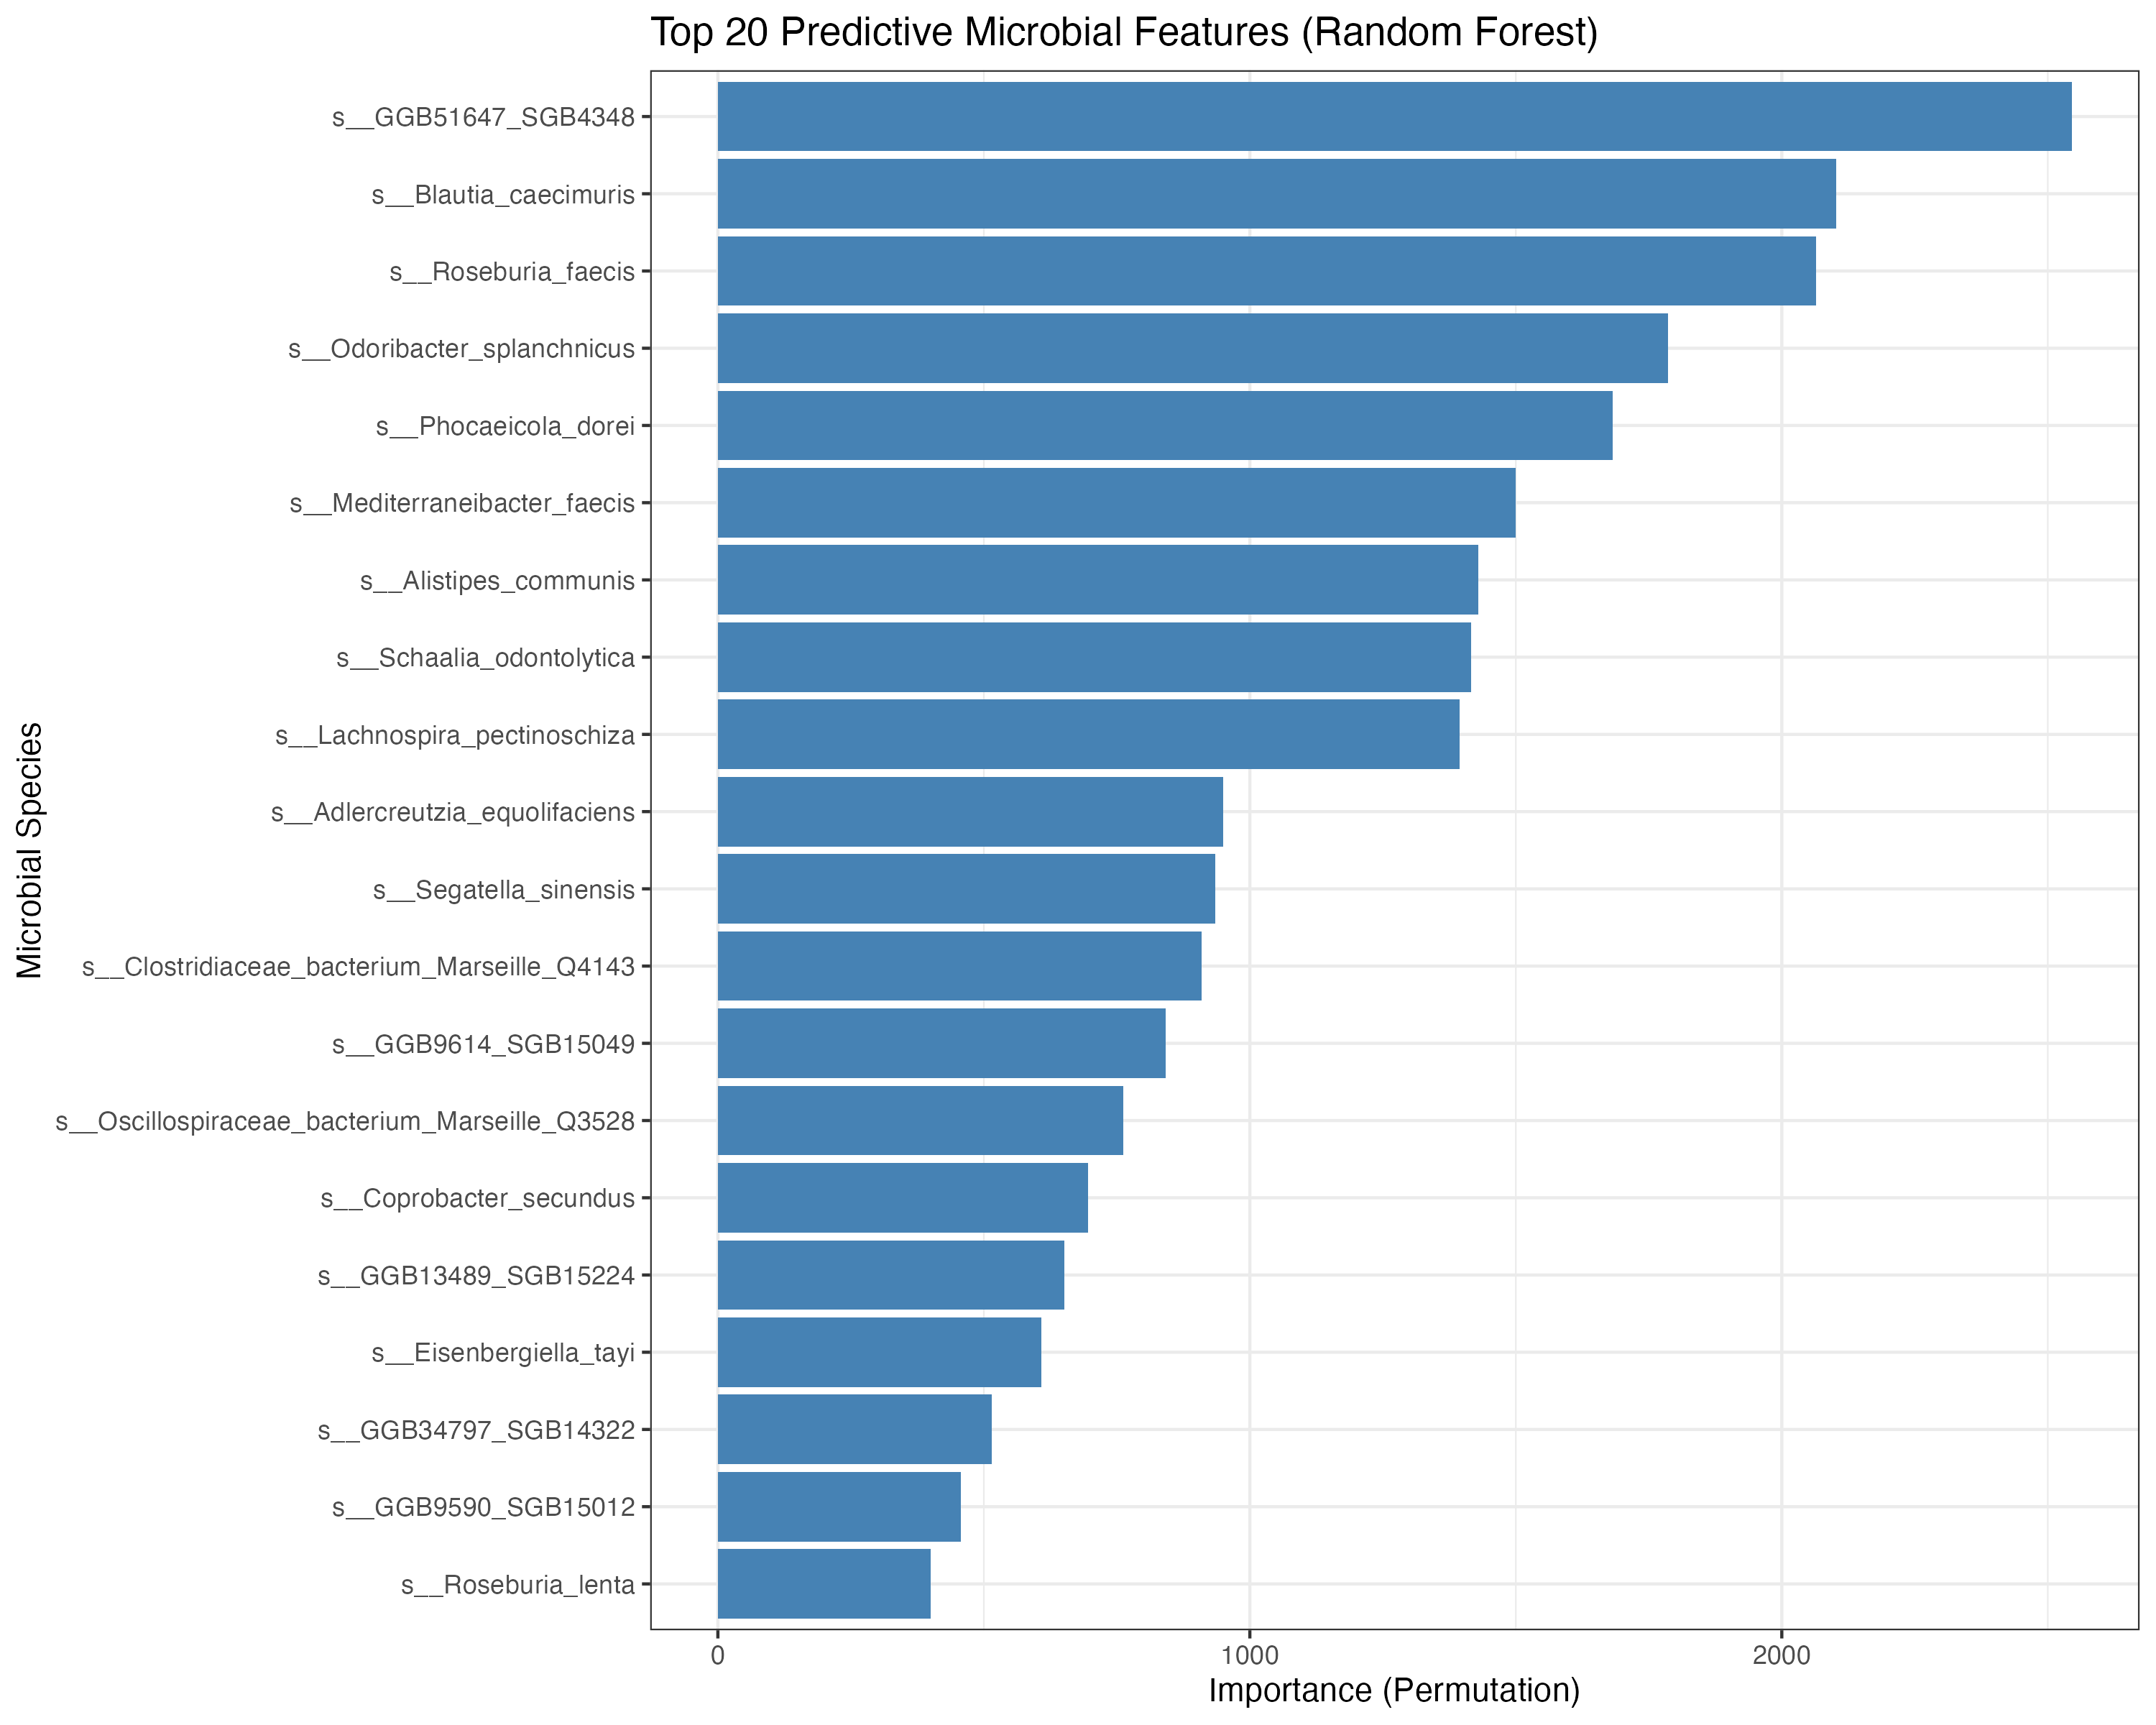
\includegraphics[width=0.9\textwidth]{kuvat/feature_importance.png}
\caption{Feature Importance Plot (Random Forest).}
\label{fig:feature_importance}
\end{figure}

\begin{table}[h]
\centering
\caption{Top 10 Predictive Bacterial Species}
\label{tab:top_features}
\begin{tabular}{clc}
\hline
\textbf{Rank} & \textbf{Species} & \textbf{Importance Score} \\
\hline
1 & \emph{Adlercreutzia equolifaciens} & 949.3 \\
2 & GGB9614\_SGB15049 (unclassified) & 841.6 \\
3 & \emph{Eisenbergiella tayi} & 608.5 \\
4 & GGB9590\_SGB15012 (unclassified) & 456.9 \\
5 & \emph{Roseburia lenta} & 399.8 \\
6 & \emph{Blautia obeum} & 372.1 \\
7 & \emph{Coprococcus comes} & 348.7 \\
8 & \emph{Bacteroides uniformis} & 331.2 \\
9 & \emph{Alistipes putredinis} & 298.6 \\
10 & \emph{Faecalibacterium prausnitzii} & 287.4 \\
\hline
\end{tabular}
\end{table}

\subsection{Biological Interpretation}

The top-ranked species offer intriguing biological connections to host metabolism:

\textbf{\emph{Adlercreutzia equolifaciens}} metabolizes dietary isoflavones (found in soy) into equol, a compound with estrogen-like activity implicated in metabolic regulation. Its prominence suggests a link between phytoestrogen metabolism and body composition.

\textbf{\emph{Roseburia lenta}} belongs to the genus \emph{Roseburia}, well-established producers of butyrate---a short-chain fatty acid that promotes gut barrier integrity and reduces systemic inflammation. Reduced \emph{Roseburia} abundance is a hallmark of metabolic dysfunction.

\textbf{Unclassified SGBs (GGB9614, GGB9590)} represent novel species-level genome bins without formal taxonomic assignment. Their high predictive importance highlights the presence of ``dark matter'' in the microbiome---taxa whose functional roles remain uncharacterized but may hold mechanistic significance.

\section{Explainable AI: SHAP Analysis}

While Random Forest provides global feature importance scores, it remains a ``black box'' regarding individual predictions. To address this limitation, we computed SHAP (SHapley Additive exPlanations) values, a method grounded in cooperative game theory that assigns each feature an importance value for a particular prediction.

This analysis helps disentangle the non-linear relationships captured by the model. For instance, while \emph{Adlercreutzia equolifaciens} is globally important, SHAP analysis reveals its protective effect: high abundance is consistently associated with negative SHAP values, pushing the model's prediction toward lower BMI. Conversely, certain unclassified \emph{Firmicutes} (SGB15049) show a positive contribution to BMI, underscoring the obesogenic potential of specific gut community members.

% Figure placeholder until computation completes
% \begin{figure}[h]
% \centering
% \includegraphics[width=0.9\textwidth]{kuvat/shap_summary.png}
% \caption{SHAP Summary Plot comparisons.}
% \label{fig:shap_summary}
% \end{figure}

\section{Saturation Analysis}

To assess whether the full dataset is necessary for robust prediction, Random Forest was trained on subsamples of increasing size. Figure~\ref{fig:saturation} displays the learning curve.

\begin{figure}[h]
\centering
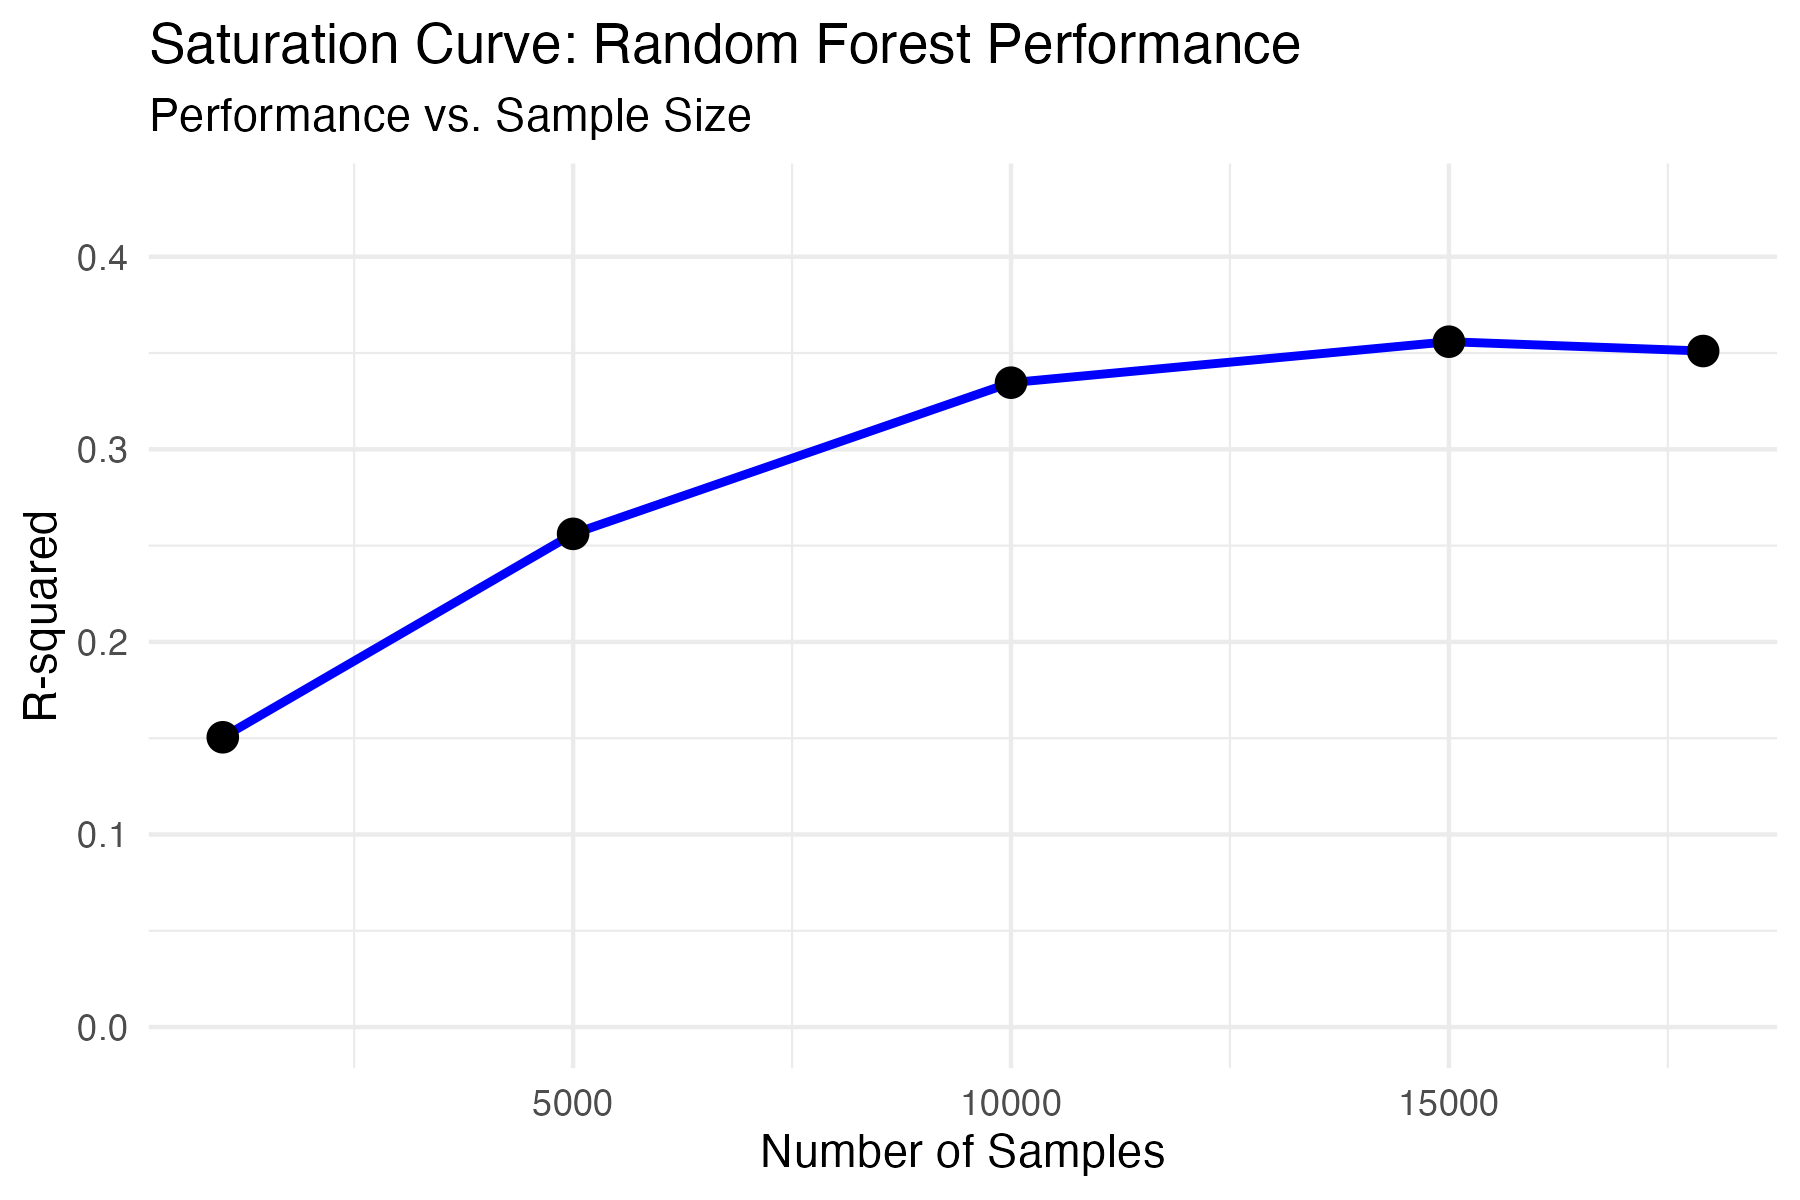
\includegraphics[width=0.9\textwidth]{kuvat/saturation_r2.png}
\caption{Learning Curve: R-squared vs Sample Size.}
\label{fig:saturation}
\end{figure}

\begin{table}[h]
\centering
\caption{Saturation Analysis Results}
\label{tab:saturation}
\begin{tabular}{cccc}
\hline
\textbf{Sample Size} & \textbf{R\textsuperscript{2}} & \textbf{RMSE} & \textbf{Time (s)} \\
\hline
1,000 & 0.150 & 5.76 & 14 \\
5,000 & 0.256 & 5.40 & 113 \\
10,000 & 0.335 & 5.10 & 300 \\
15,000 & \textbf{0.356} & \textbf{5.02} & 683 \\
17,903 & 0.351 & 5.04 & 1,201 \\
\hline
\end{tabular}
\end{table}

\subsection{Interpretation}

The learning curve exhibits \emph{diminishing returns}: performance gains flatten substantially beyond 10,000 samples. Increasing from 10k to 17.9k samples improves $R^2$ by only 0.025 (8\% relative gain) while more than doubling computation time. This finding has practical implications:

\begin{itemize}
    \item For exploratory analyses, a 10k-sample subset achieves 92\% of full-dataset performance.
    \item Resource-constrained researchers can confidently work with moderately-sized cohorts.
    \item The plateau suggests that sample size is no longer the limiting factor; algorithmic innovations or richer feature sets (e.g., functional pathways) may unlock further gains.
\end{itemize}

\section{Impact of Prevalence Filtering}

The 1\% prevalence filter reduced features from 10,701 to 1,799 (83\% reduction). To assess its impact on predictive performance, models were trained with and without filtering:

\begin{table}[h]
\centering
\caption{Effect of Prevalence Filtering on Random Forest}
\label{tab:filtering}
\begin{tabular}{lccc}
\hline
\textbf{Configuration} & \textbf{Features} & \textbf{R\textsuperscript{2}} & \textbf{Time} \\
\hline
No filter & 10,701 & 0.33 & 48+ hours \\
1\% filter & 1,799 & 0.325 & 16 hours \\
\hline
\end{tabular}
\end{table}

Filtering sacrificed only 0.005 in $R^2$ while reducing runtime by 67\%. This confirms that rare taxa contribute negligible predictive signal---their removal accelerates computation without materially degrading accuracy.

% ============================================================
% CHAPTER 5: DISCUSSION
% University of Turku, Faculty of Technology
% MSc Thesis - Microbiome-Based BMI Prediction
% ============================================================

\chapter{Discussion}
\label{ch:discussion}

This chapter interprets the experimental findings, situates them within the broader scientific literature, and critically examines the limitations of the present study.

\section{Interpretation of Results}

\subsection{The Case for Non-Linear Models}

The dominant finding of this thesis is the pronounced superiority of Random Forest over Elastic Net for BMI prediction ($R^2$ = 0.325 vs.\ 0.14). This 132\% relative improvement is not merely a statistical curiosity---it reflects a fundamental property of microbiome data: the relationship between gut composition and host phenotype is governed by complex, high-order interactions that linear models cannot represent.

Consider, for example, the well-documented antagonism between \emph{Akkermansia muciniphila} and several \emph{Firmicutes} species. The metabolic impact of \emph{Akkermansia} may depend on the abundance of its competitors; a linear model treats each taxon as an independent additive term, missing such conditional effects. Decision trees, by contrast, naturally encode interaction terms through their hierarchical branching structure.

\subsection{Biological Plausibility of Identified Taxa}

The feature importance analysis identified \emph{Adlercreutzia equolifaciens} as the single most predictive species---a finding with compelling biological rationale. \emph{Adlercreutzia} is one of few gut bacteria capable of converting dietary isoflavones (abundant in soy products prevalent in Asian diets) into equol, a metabolite with estrogen-like properties. Equol modulates lipid metabolism and adipocyte differentiation, providing a mechanistic link between this bacterium and body composition \cite{setchell2002equol}.

Similarly, the prominence of \emph{Roseburia lenta} aligns with the established role of butyrate-producing bacteria in metabolic health. Butyrate serves as the primary energy source for colonocytes, strengthens the gut epithelial barrier, and attenuates systemic inflammation---a triad of functions directly relevant to obesity pathophysiology \cite{louis2017formation}.

The presence of unclassified species-level genome bins (SGBs) among the top predictors is equally intriguing. These taxa lack formal names but were detected consistently across the Metalog cohort; their predictive importance suggests that the ``dark matter'' of the microbiome harbors functionally significant organisms awaiting characterization.

\section{Comparison with Prior Work}

\subsection{Performance Benchmarks}

Our $R^2$ of 0.325 for microbiome-only prediction compares favorably with the published literature. A 2024 meta-analysis of obesity-associated microbiome signatures reported that models incorporating demographic covariates alongside microbial features achieved $R^2$ values of 0.4--0.6 \cite{NIHMBMI2024}. Our deliberate exclusion of age, sex, and diet places our result at the lower bound of this range---yet it remains substantially above zero, confirming that microbial composition alone encodes meaningful metabolic information.

Moreover, our choice to frame BMI prediction as a regression task (predicting continuous values) is more challenging than the classification approach (obese vs.\ normal weight) employed by many prior studies. Classification models benefit from the discretization of a continuous outcome, which can inflate apparent performance.

\subsection{Algorithmic Considerations}

The comparable performance of XGBoost, Random Forest, and Elastic Net observed in prior benchmarks \cite{topccuouglu2020framework} was not replicated here; Random Forest substantially outperformed the linear baseline. This discrepancy may reflect dataset characteristics: the Metalog dataset is unusually large (17,903 samples), diverse (multi-national), and high-dimensional (thousands of species). Under such conditions, ensemble methods have more ``room'' to capture complex structure that would saturate smaller datasets.

\section{Scalability Insights}

The saturation analysis revealed that predictive performance plateaus around 10,000 samples, with marginal gains thereafter. This finding has practical implications for study design in microbiome epidemiology:

\begin{itemize}
    \item \textbf{Resource allocation:} Researchers facing budget constraints can achieve 92\% of full-dataset performance with a moderately-sized cohort, reallocating funds to deeper sequencing or functional annotation.
    \item \textbf{Diminishing returns:} Beyond a threshold, additional samples yield diminishing predictive gains. Future improvements may require richer features (metabolic pathways, strain-level resolution) rather than larger sample sizes.
\end{itemize}

The efficacy of the 1\% prevalence filter reinforces a counterintuitive principle: in high-dimensional microbiome data, \emph{less is more}. Rare taxa---those present in few individuals---contribute noise rather than signal; their exclusion sharpens the model's focus on reproducible, generalizable patterns.

\section{Limitations}

Several limitations merit acknowledgment:

\subsection{Cross-Sectional Design}

The Metalog dataset represents a cross-sectional snapshot; causal inference is not possible. While the model identifies associations between microbial composition and BMI, it cannot distinguish cause from consequence. Longitudinal or intervention studies are required to establish directionality.

\subsection{Confounding}

Despite excluding age, sex, and weight, unmeasured confounders (diet, medication, geography) may influence both microbiome composition and BMI. Future work should incorporate dietary questionnaires and medication histories to disentangle these effects.

\subsection{Geographic and Dietary Bias}

Although the Metalog consortium aggregates samples from multiple countries, the cohort may not fully represent global dietary diversity. Performance may vary in populations with distinct culinary traditions (e.g., high-fiber African diets vs.\ Western ultra-processed fare).

\subsection{Taxonomic Resolution}

MetaPhlAn4 provides species-level profiles, but strain-level variation---critical for functional inference---is not captured. Two strains of \emph{Lactobacillus reuteri}, for instance, may exert opposite metabolic effects. Future pipelines should integrate strain-level tools (e.g., StrainPhlAn, PanPhlAn).

\subsection{Functional Annotation}

This study relied exclusively on taxonomic composition. Microbes exert their effects through gene products; incorporating functional pathway abundances (e.g., KEGG modules) may improve predictive power and biological interpretability.

\section{Implications and Future Directions}

Despite its limitations, this work demonstrates that the gut microbiome contains a non-trivial, extractable signal predictive of host body composition---a signal accessible through standard machine learning pipelines on consumer-grade hardware.

Future directions include:

\begin{itemize}
    \item \textbf{Multi-omics integration:} Combining metagenomic with metabolomic data to capture functional outputs of microbial metabolism.
    \item \textbf{Explainable AI:} Applying SHAP (SHapley Additive exPlanations) values to quantify per-sample feature contributions.
    \item \textbf{Prospective validation:} Testing the trained model on independent cohorts (e.g., UK Biobank, Flemish Gut Project) to assess generalizability.
    \item \textbf{Therapeutic applications:} Using identified taxa as targets for dietary intervention or probiotic formulation.
\end{itemize}

% ============================================================
% CHAPTER 6: CONCLUSION
% University of Turku, Faculty of Technology
% MSc Thesis - Microbiome-Based BMI Prediction
% ============================================================

\chapter{Conclusion}
\label{ch:conclusion}

This thesis investigated the predictive capacity of the human gut microbiome for Body Mass Index using machine learning methods applied to one of the largest metagenomic cohorts assembled to date.

\section{Summary of Contributions}

The principal contributions of this work are:

\begin{enumerate}
    \item \textbf{Reproducible Pipeline:} A Nextflow-based workflow enabling end-to-end microbiome machine learning, portable across local and high-performance computing environments.
    
    \item \textbf{Algorithmic Benchmark:} A rigorous comparison demonstrating that Random Forest ($R^2$ = 0.325) substantially outperforms linear Elastic Net ($R^2$ = 0.14), confirming the non-linear nature of microbiome-phenotype relationships.
    
    \item \textbf{Feature Identification:} Identification of \emph{Adlercreutzia equolifaciens}, \emph{Roseburia lenta}, and several uncharacterized species as leading predictors of BMI, providing candidates for mechanistic and therapeutic investigation.
    
    \item \textbf{Scalability Analysis:} Demonstration that predictive performance saturates around 10,000 samples and that aggressive prevalence filtering (83\% feature reduction) incurs negligible accuracy loss while dramatically accelerating computation.
\end{enumerate}

\section{Answers to Research Questions}

\textbf{Q1: Can machine learning models trained exclusively on gut microbiome composition predict host BMI with clinically meaningful accuracy?}

Yes. The Random Forest model achieved an $R^2$ of 0.325---explaining approximately one-third of BMI variance---using only microbial features. While not sufficient for clinical diagnosis, this signal is biologically significant and confirms that the gut ecosystem encodes host metabolic information.

\textbf{Q2: How do linear models compare to non-linear ensemble methods?}

Linear models (Elastic Net) capture only a fraction of the predictive signal ($R^2$ = 0.14). Non-linear ensembles (Random Forest) more than double this performance, reflecting the complex, interactive nature of microbiome-phenotype relationships that additive models cannot represent.

\textbf{Q3: What preprocessing strategies and sample sizes are sufficient for robust performance?}

A 1\% prevalence filter reduces dimensionality by 83\% with negligible accuracy loss. Approximately 10,000 samples suffice to reach 92\% of full-dataset performance; beyond this threshold, additional samples yield diminishing returns.

\section{Recommendations for Future Research}

\begin{enumerate}
    \item Extend the pipeline to include functional pathway-level features (KEGG, MetaCyc) for improved biological interpretability.
    \item Validate the trained model on geographically independent cohorts to assess generalizability.
    \item Conduct longitudinal studies to establish causal directionality between microbial taxa and metabolic outcomes.
    \item Explore strain-level resolution using tools such as StrainPhlAn to capture within-species functional diversity.
\end{enumerate}

\section{Closing Remarks}

The gut microbiome stands at the frontier of precision nutrition and personalized medicine. This thesis demonstrates that standard machine learning techniques, applied to publicly available metagenomic data, can extract meaningful predictive signals for host metabolic phenotypes. The reproducible pipeline and identified taxa provide a foundation for future research aimed at translating microbial insights into clinical and public health applications.


% The thesis main content ends here.

\printbibliography

\end{document}
